\documentclass{elsart}
\usepackage[numbers]{natbib}
\usepackage[dvips]{graphicx}

\newcommand{\threej}[6]{\ensuremath{\left({#1\atop #4}{#2\atop #5}
{#3\atop #6}\right)}}
\newcommand{\sixj}[6]{\ensuremath{\left\{{#1\atop #4}{#2\atop #5}
{#3\atop #6}\right\}}}

\newcommand{\pra}{Phys. Rev. A}
\newcommand{\cpc}{Comput. Phys. Commun.}
\newcommand{\jpb}{J. Phys. B}
\newcommand{\ant}{At. Data Nucl. Data Tables}
\newcommand{\amp}{Adv. Atom. Mol. Phys.}
\newcommand{\aaa}{Astron. Astrophys.}
\newcommand{\apjs}{ApJ. Suppl.}
\newcommand{\apj}{ApJ.}
\newcommand{\jqsrt}{J. Quant. Spectros. Rad. Transf.}

\defcitealias{gu01a}{Paper~I}
\defcitealias{gu01b}{Paper~II}
\defcitealias{gu01c}{Paper~III}
\defcitealias{gu01d}{Paper~IV}

\begin{document}

\begin{frontmatter}

\title{Flexible Atomic Code: V. Electron Impact Ionization}  
\author{Ming Feng Gu}
\address{Massachusetts Institute of Technology, Cambridge, MA 02139, USA}

\begin{abstract} 
The detailed level-to-level electron impact ionization cross sections are
calculated in the relativistic distorted-wave approximation, extending the 
factorization-interpolation method developed for the calculation of electron
impact excitation cross sections. The implementation allows for the most
general configuration mixing to be included. Total 
direct ionization cross sections from the ground state of Ne-like Fe
are calculated, and compared with a previously published work using
the non-relativistic distorted-wave approximation. 
\end{abstract}

\begin{keyword}
Distorted-wave \sep Electron impact ionization.
\PACS 34.80.Kw
\end{keyword}

\end{frontmatter}

\textbf{\large PROGRAM SUMMARY}

Title of program: FAC

Catalogue identifier:

Distribution formate:

Computer for which the program is designed and others on which the program has
been tested:\\
Computers: Sun Workstations, PCs\\
Operating systems under which the program has been tested: Unix

Programming language used: C, Fortran, Python

Number of bits in a word: 64

Number of processors used: 1

Has the code been vectorized or parallelized: No

Keywords: Distorted-wave, Electron impact ionization.

Nature of physical problem: Direct ionization by electron impact is an
important process determining the ionization balance of hot plasmas. The
ionization of inner-shell electrons may also lead to the formation of spectral
lines. 

Method of solution: Extending the factorization-interpolation method used in
the distorted-wave theory of electron impact excitation, direct ionization by
electron impact is treated in the relativistic distorted-wave approximation.  

Restrictions on the complexity of program: No special restrictions except for
that of system resources. 

Typical running time: The test run takes 3 min on an Ultra 10 Sun workstation.

\textbf{\large LONG WRITE-UP}

\section{Introduction}
This is the fifth paper of a sequence describing a systematic software
package, the Flexible Atomic Code (FAC), 
for calculating atomic radiative and collisional processes in the relativistic
distorted-wave (DW) approximation. In the previous papers
(\citetalias{gu01a}\citep{gu01a},\citetalias{gu01b}\citep{gu01b},
\citetalias{gu01c}\citep{gu01c}, and \citetalias{gu01d}\citep{gu01d}), the
calculation of atomic structure, electron impact excitation (EIE),
non-resonant photoionization and radiative recombination, autoionization and
dielectronic recombination are discussed. This paper deals with the direct
ionization by electron impact (EII). Accurate EII cross sections are needed
to calculate the ionization balance in the modeling of hot plasmas. Inner
shell EII is also important as an emission line formation process. 

Several DW programs have been developed for the calculation of EII cross
sections in the past decades, in either non-relativistic \citep{younger80} or
relativistic \citep{pindzola88, sampson91} approximations. The present program
is similar to that of 
\citet{sampson91} in particular,  which extends the
efficient factorization-interpolation method of \citet{barshalom88} to the
calculation of EII cross sections, and leads to great simplifications for
complex ions. The essence of the factorization method is the separation of
the angular and radial parts in the formula of EII cross sections. The angular
part depends on the angular momentum coupling of the target states, while the
radial part only depends on the one-electron radial orbitals, without
explicit reference to the initial and final states involved in the
process. Different initial and final states affect the radial part only
implicitly through the ionization energy due to the energy conservation. Such
a separation enables the rapid calculation of the radial integrals on a few
ionization energy points, the integrals at actual ionization energies are
obtained by interpolation.  

This paper is organized as following. 
\S\ref{sec_theory} presents a brief theoretical background and some important
numerical techniques used in the program. \S\ref{sec_program} introduces the
FAC routines relevant to the calculation of EII cross
sections. \S\ref{sec_example} illustrates the practical usage of these
routines through an example, and compares the present 
results to the previous work.

\section{Theory and Numerical Techniques}
\label{sec_theory}
The formula for EII cross section, differential in energy of the ejected
electron, may be obtained from that for EIE by replacing one bound orbital in
the final state with the free orbital of the ejected electron and summing 
over its angular momentum. It can be expressed in terms of the collision
strength similar to that of EIE 
\begin{equation}
\label{eq_cross}
\sigma(\varepsilon_0,\varepsilon) = \frac{1}{k_0^2g_0}\Omega_{01},
\end{equation}
where $\varepsilon_0$ and $k_0$ are the energy and kinetic momentum of the
incident electron, $\varepsilon$ is the energy of the ejected electron. The
normalization of continuum orbitals is discussed in \citetalias{gu01b}. Note
that the absence of the 
factor $\pi$ as compared with the formula for the EIE cross section is due to
the different normalization of the free and bound orbitals. The collision
strength $\Omega_{01}$ is \citep{gu01b}
\begin{eqnarray}
\label{eq_cs}
\Omega_{01} &=& 2\sum_{\kappa,J_T}\sum_{k}\sum_{\alpha_0\beta_0}
Q^k(\alpha_0\kappa;\beta_0\kappa)\times \nonumber\\ 
&&<\psi_0||Z^k(\alpha_0,\kappa)||\psi_1,\kappa;J_T>
<\psi_0||Z^k(\beta_0,\kappa)||\psi_1,\kappa;J_T>,
\end{eqnarray}
where $\kappa$ is the relativistic angular quantum number of the ejected
electron, $J_T$ is the total angular momentum of the final state coupled with
the ejected electron,
the radial part $Q^k$ is identical to that for EIE, except that one of
the bound orbitals in the final state is now replaced by a free orbital. Note
that $Q^k$ contains the summation over the partial waves of incident and
scattered electrons.

As for photoionization \citep{gu01b}, the angular factors involving the free
electron can be simplified using the decoupling formula of Racah
\begin{eqnarray}
&<&\psi_0||Z^k(\alpha_0, \kappa)||\psi_1,\kappa;J_T>
<\psi_0||Z^k(\beta_0, \kappa)||\psi_1,\kappa;J_T> = \nonumber\\
&<&\psi_1||\tilde{a}_{\tilde{\alpha_0}}||\psi_0>
<\psi_1||\tilde{a}_{\tilde{\beta_0}}||\psi_0>
\sum_{J_T}[J_T]\sixj{J_1}{j}{J_T}{k}{J_0}{j_{\alpha_0}}
\sixj{J_1}{j}{J_T}{k}{J_0}{j_{\beta_0}},
\end{eqnarray}
where $[J_T]$ denotes $2J_T+1$ and $\sixj{j_1}{j_2}{j_3}{j_4}{j_5}{j_6}$ is
the Wigner $6j$ symbol. 
Substituting this into Equation \ref{eq_cs}, and carrying
out the summation over $J_T$ analytically, we find
\begin{equation}
\Omega_{01} = 2\sum_{k,\alpha_0\beta_0}
\delta_{j_{\alpha_0}j_{\beta_0}}[j_{\alpha_0}]^{-1} 
\overline{Q}^k(\alpha_0,\beta_0)
<\psi_1||\tilde{a}_{\tilde{\alpha_0}}||\psi_0>
<\psi_1||\tilde{a}_{\tilde{\beta_0}}||\psi_0>,
\end{equation}
where $\overline{Q}^k(\alpha_0,\beta_0) = \sum_\kappa
Q^k(\alpha_0\kappa;\beta_0\kappa)$.
Note that since only basis states with the same parity can mix, the condition
$j_{\alpha_0}=j_{\beta_0}$ implies that $l_{\alpha_0} = l_{\beta_0}$ as
well. Therefore, if the configuration interaction is limited within the same
$n$ complex, only terms with $\alpha_0 = \beta_0$ survive in the summation. 

The total ionization cross section is obtained by integrating $\Omega_{01}$
over the energy of the ejected electron, $\varepsilon$
\begin{equation}
\label{eq_total}
\sigma(\varepsilon_0) = \int\nolimits_0^{\frac{\varepsilon_0-I}{2}}
\sigma(\varepsilon_0,\varepsilon) \d\varepsilon,
\end{equation}
where $I$ is the ionization energy. The ionization energy enters the
radial integral $Q^k$ implicitly, since $\varepsilon_0 =
I+\varepsilon_1+\varepsilon$, where $\varepsilon_1$ is the energy of the
scattered electron. We choose to calculate $Q^k$ as a function of $I$,
$\varepsilon_1$, and $\varepsilon$. For a given transition array, we first set
up a three dimensional grid on these three energies. The integrals $Q^k$ are 
only calculated on this grid, values for arbitrary energies are obtained by
interpolation. For a given ionization channel with
ionization energy of $I_{01}$ and the incident electron energy of
$\varepsilon_t + I_{01}$, where $\varepsilon_t$ is the sum of the energies of
the two final electrons, the calculation of the total cross section proceeds as
following. The first step is the interpolation on the $I$ grid to obtain, for
each point on the $(\varepsilon_1,\varepsilon)$ grid, the values of
$\overline{Q}^k(I_{01})$ at the actual ionization energy, $I_{01}$. We then
establish another grid for the energy of the ejected electron in the range 
from 0 to $\varepsilon_t/2$ for the purpose of the numerical integration in
Equation \ref{eq_total}. For each 
point on this grid, the value of $\varepsilon_1 = \varepsilon_t-\varepsilon$
is determined. A two dimensional interpolation is then performed on the array
$\overline{Q}^k(I_{01},\varepsilon_1,\varepsilon)$ to obtain the radial
integrals at these specific 
energies. Finally the integral in Equation \ref{eq_total} is evaluated to
yield the total cross section. In practice, we find such a procedure
minimizes the number of radial integrals need to be computed explicitly. The
number of grid points for the ionization energy is chosen similarly as for the
excitation energies of EIE, that is, 2 points with linear interpolation when
the ionization energies vary by less than 20\%, and 3 points with cubic spline
interpolation otherwise. The grids for the $\varepsilon_1$ and $\varepsilon$
are usually chosen to have 6 points spanning the range necessary to cover the
collision energies where the total cross sections are needed.

For each point on the three dimensional grid $(I,\varepsilon_1, \varepsilon)$,
and bound orbitals $\alpha_0$ and $\beta_0$, the evaluation of
$\overline{Q}^k(\alpha_0,\beta_0)$ involves the summation of the 
partial waves of all free electrons. The angular momentum of the ejected
electron must satisfy the triangular relation $\Delta(j_{\alpha_0}, k, j)$,
therefore, the limit on the rank $k$ in the expansion of the Coulomb
interaction restricts the number of $\kappa$ terms. Usually $k_{max} = 6$ is
large enough to ensure the convergence. A further limit on the orbital angular
momentum of 
the ejected electron may also be specified. The summation over the partial
waves of the incident and scattered electrons proceeds exactly the same way as
in the calculation of EIE cross sections, using the Coulomb-Bethe
approximation for the high partial waves in the case of allowed integrals.

\section{User Interface}
\label{sec_program}
The general features of the FAC user interface and that related to the other
parts of FAC are discussed in the previous papers
I--IV\citep{gu01a,gu01b,gu01c,gu01d}. The Python routines relevant to the
calculation of EII cross 
sections are very similar to those for the calculation of EIE cross sections. 

The optional routines ``SetCIPWOptions'', ``SetCIPWGrid'', ``SetIEGrid'', and
``SetCIEGrid'' have similar calling syntax as their counterparts in the EIE
calculations, ``SetCEPWOptions'', ``SetCEPWGrid'', ``SetTEGrid'', and
``SetCEGrid'', respectively, except for ``SetCIPWOptions'', which accepts one
more optional parameter specifying the maximum orbital angular
momentum of the ejected electron. The calling sequence of this routine is now
``SetCIPWOptions(eps, lmax, lmax\_eject, qr)'', where ``lmax\_eject'' is the
maximum orbital angular momentum of the ejected electron, other parameters are
the same as in ``SetCEPWOptions''. The default value for ``lmax\_eject'' is 8. 

The collision energies are specified with ``SetUsrCIEGrid'', whose counterpart
in EIE is ``SetUsrCEGrid''. The energy specified is the sum of the energies of
the two final free electrons by default, unless the routine
``SetUsrCIEGridType(type)'' is called with ``type = 0'', which means the
energy specified is that of the incident electron. 

Similar to ``CETable'', ``CITable(b, f, fname)'' calculates the
ionization cross sections from all levels in ``b'' to those in ``f'',
and output the results in ``fname''. The format is similar to that of
``CETable'' as well. The collision strengths in the output are 
the integrated results over the energy of the ejected electron. The cross
sections are in the units of $10^{-20}$ cm$^2$. The routine ``SetCIFormat(m)''
may be used to indicate whether only collision strengths (m = 1), only cross
sections (m = 2) or both (m = 0) need to be output. The default is ``m = 0''.

\section{Example}
\label{sec_example}
The Python script shown below is used to calculate the cross sections of
direct ionization from the ground state of Ne-like iron. Only the ionization
of $2s$ and $2p$ subshells is included.
\begin{verbatim}
# import the modules
import fac
import config

fac.SetAtom('Fe')
# 1s shell is closed
config.closed('1s')
# Ne-like ground state
config.config('2*8', group='fe17')
# F-like configuations
config.config('2*7', group='fe18')

# solve the structure problem
fac.OptimizeRadial(['fe17', 'fe18'])
fac.Structure('fe17')
fac.Structure('fe18')
fac.LevelTable('ne_f.lev')

# set the collision energies
# 21 points with 400 eV step starting from 500 eV.
e = [500.0]
for i in range(20):
    e.append(e[i]+400.0)
fac.SetUsrCIEGrid(e)

fac.CITable(['fe17'], ['fe18'], 'ne.ci')
\end{verbatim}

The results of the present calculation are shown in Figure
\ref{fig_comparison}. The cross sections employed in the
iron ionization equilibrium calculations of \citet{arnaud92}, which are
based on the non-relativistic DW results of \citet{younger82}, are also
presented for comparison. The two sets of cross sections for the removal of
$2s$ and $2p$ subshells agree with each other to within a few percent at low
energies. At higher energies, the present results are $\sim$ 10--15\% larger,
which indicates the possible failure of convergence for the partial wave
summation in the calculaion of \citet{younger82}, where the summation was
arbitrarily truncated. 

\begin{figure}
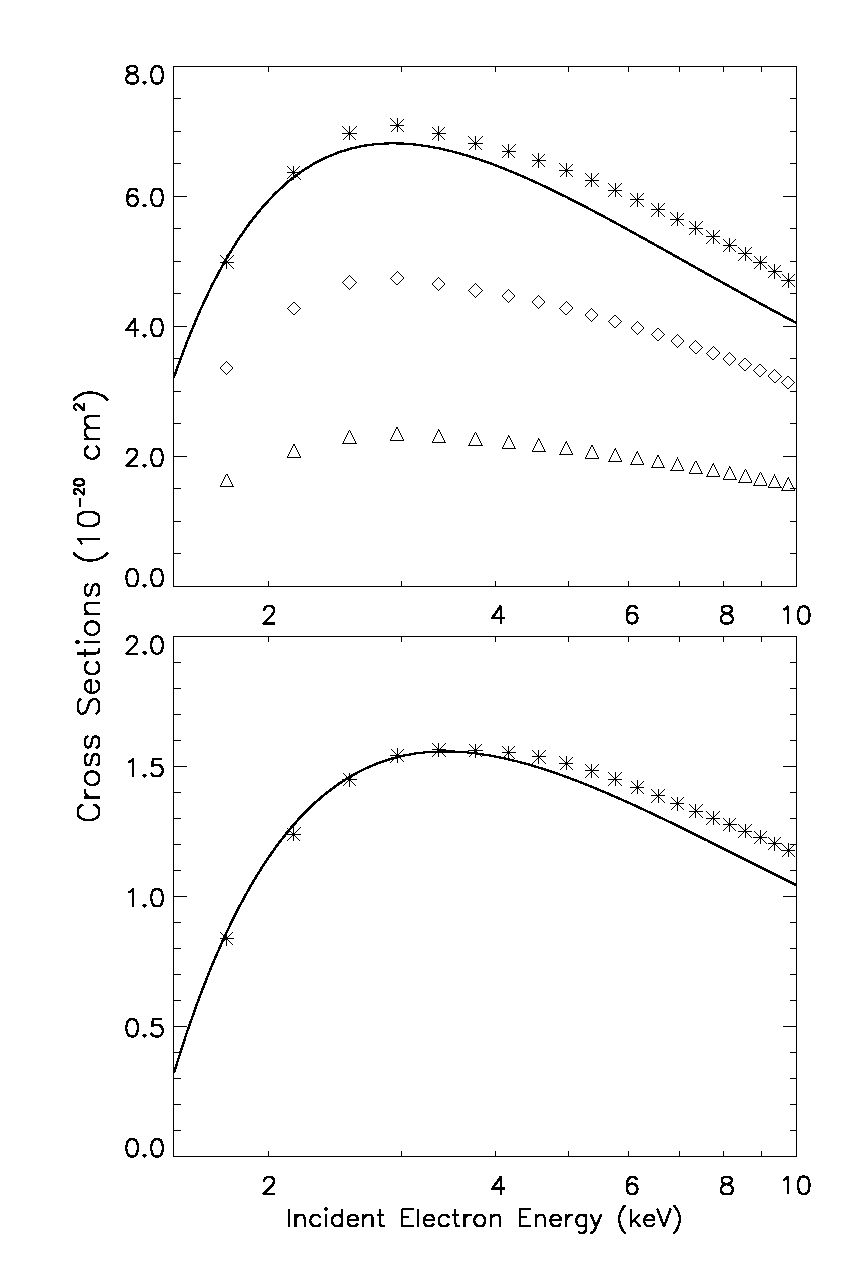
\includegraphics[width=5in]{ion0.eps}
\caption{\label{fig_comparison}Cross sections for the direct
ionization of $2s$ and $2p$ subshells of Ne-like iron. The top panel is for
the ionization of $2p$ electron, open triangles and diamonds are the
present results for the $2p_{1/2}$ and $2p_{3/2}$ subshells, respectively,
stars are the sum of the two. The bottom panel is for the ionization of $2s$
electron, stars are the present results. The solid lines in both panels are
the non-relativistic DW results of \citet{younger82} for $2p$ and $2s$
subshells.} 
\end{figure}

\section{Conclusions}
A relativistic DW program for the calculation of the direct ionization cross
sections by electron impact is described.  This program is part of the
integrated atomic software package, FAC. A factorized formula for the EII
cross section is used, and the radial integrals are calculated by an efficient
interpolation procedure. The test results for the ionization of $2s$ and $2p$
electrons of Ne-like iron show good agreement with the previous
non-relativistic DW calculations. 

\section*{Acknowledgments}
The author would like to thank Masao Sako for his continuous test of the code,
and Ehud Behar, Peter Beiersdorfer for the helpful suggestions. 
This work is supported by
NASA through Chandra Postdoctoral Fellowship Award Number PF01-10014 issued by
the Chandra X-ray Observatory Center, which is operated by Smithsonian
Astrophysical Observatory for and on behalf of NASA under contract NAS8-39073.

\bibliographystyle{unsrtnat}
\bibliography{facref}

\end{document}

